%
% File acl2012.tex
%
% Contact: Maggie Li (cswjli@comp.polyu.edu.hk), Michael White (mwhite@ling.osu.edu)
%%
%% Based on the style files for ACL2008 by Joakim Nivre and Noah Smith
%% and that of ACL2010 by Jing-Shin Chang and Philipp Koehn


\documentclass[11pt,letterpaper]{article}
\usepackage[letterpaper]{geometry}
\usepackage{acl2012}
\usepackage{times}
\usepackage{latexsym}
\usepackage{amsmath}
\usepackage{multirow}
\usepackage{graphicx}
\usepackage{todonotes}
\usepackage{url}
\makeatletter
\newcommand{\@BIBLABEL}{\@emptybiblabel}
\newcommand{\@emptybiblabel}[1]{}
\makeatother
\usepackage[hidelinks]{hyperref}
\DeclareMathOperator*{\argmax}{arg\,max}

\newcommand{\Listener}{L}
\newcommand{\Speaker}{S}
\newcommand{\utt}{u}
\newcommand{\uttlen}{N}
\newcommand{\referent}{c}
\newcommand{\context}{C}
\newcommand{\contextlen}{K}
\newcommand{\target}{t}
\newcommand{\numsamples}{m}
\renewcommand{\|}{\mid}
\newcommand{\best}[1]{\textbf{#1}}

\newcommand{\Secref}[1]{Section~\ref{#1}}
\newcommand{\secref}[1]{Section~\ref{#1}}
\newcommand{\dashsecref}[2]{Sections~\ref{#1}--\ref{#2}}
\newcommand{\Figref}[1]{Figure~\ref{#1}}
\newcommand{\figref}[1]{Figure~\ref{#1}}
\newcommand{\dashfigref}[2]{Figures~\ref{#1}--\ref{#2}}
\newcommand{\Tabref}[1]{Table~\ref{#1}}
\newcommand{\tabref}[1]{Table~\ref{#1}}
\newcommand{\pararef}[1]{\textbf{#1}}

\setlength\titlebox{6.5cm}    % Expanding the titlebox

\title{Instructions for TACL Submissions}

\author{First Author \\
  Affiliation / Address line 1 \\
  Affiliation / Address line 2 \\
  Affiliation / Address line 3 \\
  {\tt email@domain} \\\And
  Second Author \\
  Affiliation / Address line 1 \\
  Affiliation / Address line 2 \\
  Affiliation / Address line 3 \\
  {\tt email@domain} \\}

\date{}

\begin{document}
\maketitle
\begin{abstract}

asdf asdf asdf 

\end{abstract}

\section{Introduction}

\section{Task}

We compare agents on a task of language understanding in a reference game. An agent $\Listener$ is presented with a list of colors $\context = \{\referent_i, i=1..\contextlen\}$ and an utterance $\utt$ that describes the target color $\referent_\target \in \context$ in natural language. The agent does not know the index $\target$ of the target color and must guess it from $\utt$.

\section{Models}

\subsection{Classifier listener}

Our base listener agent $L_0$ is an LSTM encoder model that produces a Gaussian
distribution over colors in a transformed representation space. This representation
space is a Fourier-transformed vector as in \newcite{MonroeGoodmanPotts16_Color}, but
with a different resolution in each dimension: 2$\times$2$\times$1 instead of
3$\times$3$\times$3.

The words in the input are embedded in a 100-dimensional vector space. Word embeddings
are initialized randomly [todo: how?] and trained. The sequence of word vectors are
used as input to an LSTM with 100-dimensional hidden state, and a linear
transformation is applied to the output representation to produce a covariance matrix
and mean vector for a Gaussian distribution in color representation space. 
The Gaussian scores for each of the $\contextlen$ context colors are normalized to
produce a probability distribution over the context colors. We denote this probability
distribution by $\Listener_0(\target \| \utt, \context; \theta)$, where $\theta$ represents the
vector of parameters that define the trained model.

\subsection{Classifier speaker}\label{sec:s0}

In order to avoid enumerating an exponentially large space of possible utterances,
we also employ a probabilistic speaker model
$\Speaker_0(\utt \| \target, \context; \phi)$ to generate sets of alternative
utterances for each context.

The speaker model consists of a recurrent neural network (RNN) context encoder
and an RNN description decoder. In this model, the colors of the context
$\referent_i \in \context$ are transformed into the Fourier representation space
of \newcite{MonroeGoodmanPotts16_Color} (we use the original 3$\times$3$\times$3
basis for the speaker model), and the sequence of color
representations is passed through a "vanilla" recurrent neural network
[todo: write out math] with 100-dimensional hidden state.

The output of this recurrent neural network is concatenated with a
100-dimensional embedding for the previous token at each time step in decoding.
The resulting vector is input along with the previous cell state to a "vanilla" RNN
cell, and an affine transformation and softmax function are applied to the output to
produce a probability distribution predicting the following token of the description.

\subsection{Pragmatic listener}

From the base classifier listener, we build a listener agent that performs
pragmatic inference using an embedded speaker model. This agent is based on the
pragmatic listener of \newcite{BergenLevyGoodman15_Reasoning}, denoted
$\Listener(\Speaker(\Listener_0))$: a listener modeling a speaker modeling the
base listener.

Formally, our pragmatic listener $\Listener_2$ is defined in terms of the base
listener as follows:
\begin{align}
\Speaker_1(\utt \| \target, \context; \theta) &\propto \Listener_0(\target \| \utt, \context; \theta)^\alpha \label{eq:s1} \\
\Listener_2(\target \| \utt, \context; \theta) &\propto \Speaker_1(\utt \| \target, \context; \theta) \nonumber
\end{align}
In practice, computing the constant of proportionality in \eqref{eq:s1} requires
enumerating over space of potential utterances that is exponentially large in the
maximum utterance length. As mentioned in \secref{sec:s0}, we limit this search by
taking $\numsamples = 3$ samples from $\Speaker_0(\utt \| i, \context; \phi)$ for
each possible target index $i$, adding the actual utterance from the testing example,
and taking the resulting set as the universe of possible utterances for the
proportionality in \eqref{eq:s1}.

We find we can obtain an additional small improvement in listener accuracy
by blending the pragmatic listener with the base listener:
\[\Listener^{*}(\target \| \utt, \context; \theta) \propto {\Listener_0}(\target \| \utt, \context; \theta)^{\beta} \cdot \Listener_2(\target \| \utt, \context; \theta)^{1-\beta}\]

\section{Corpus collection}

\begin{figure}
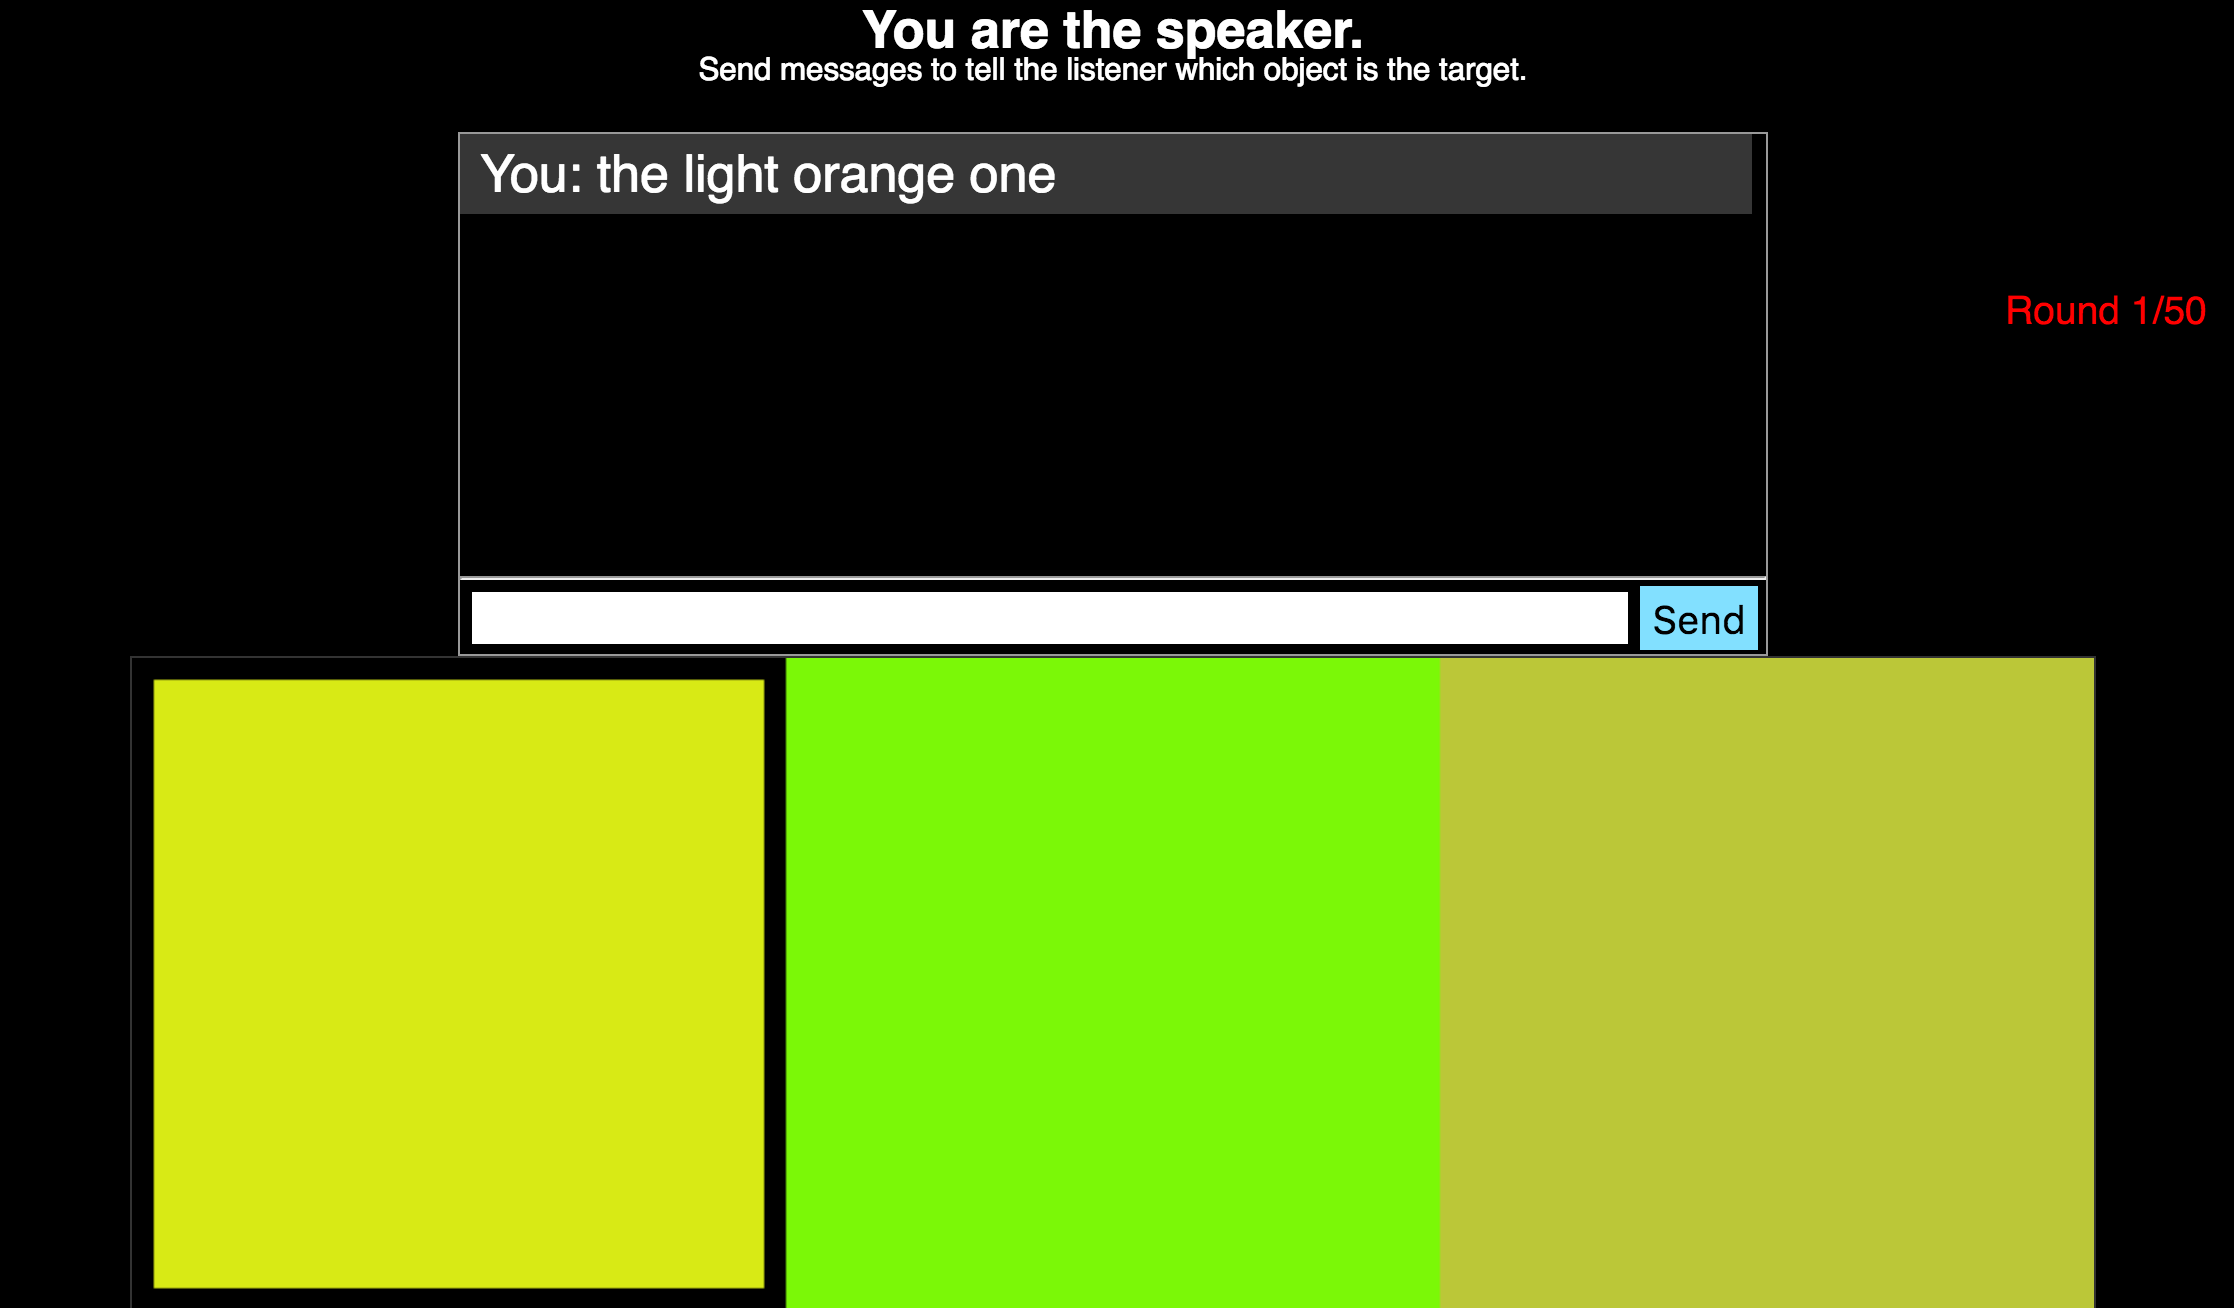
\includegraphics[scale = .2]{figures/speakerView.png}
\caption{Example trial in corpus collection task, from speaker's perspective}
\label{fig:taskScreenshot}
\end{figure}

To collect a corpus of natural color reference data across varying contexts, we recruited 210 participants from Amazon Mechanical Turk to play a real-time, multi-player communication game \cite{Hawkins15_RealTimeWebExperiments}. Participants were sorted into dyads, assigned the role of speaker or listener, and placed in a game environment containing a chat box and an array of three color patches (Fig. \ref{fig:taskScreenshot}). 

On each round, one of the three colors was chosen to be the ``target'' and highlighted for the speaker. They were instructed to communicate this information to the listener, who could then click on one of the colors to advance to the next trial. Both participants were free to use the chat box at any point during the trial. 

To ensure a range of difficulty, we randomly interspersed an equal number of trials from three different conditions: (1) \emph{close}, where colors were all within a distance of $\theta$ from one another but still perceptible\footnote{We used the most recent CIEDE standard to measure color differences, which is calibrated to human vision \cite{SharmaWuDalal05_DeltaE}. All distances were constrained to be larger than a lower bound of $\epsilon = 5$ to ensure perceptible differences, and we used a threshold value of $\theta = 20$ to create conditions}, (2) \emph{split}, where one distractor was within a distance of $\theta$ of the target, but the other distractor was further than $\theta$, and (3) \emph{far}, where all colors were farther than $\theta$ from one another. Colors were rejection sampled uniformly from RGB space to meet these constraints. 

% latex table generated in R 3.3.0 by xtable 1.8-2 package
% Wed Oct  5 12:20:44 2016
\begin{table*}[t]
\centering
\begin{tabular}{lrrr|rrr}
  & \multicolumn{3}{c}{human}& \multicolumn{3}{c}{model}\\ \hline
  & far& close& split& far& close& split\\ \hline
\# Chars & 13.12 & 11.87 & 8.17 & 7.14 & 6.00 & 5.21 \\ 
  \# Comparatives & 0.13 & 0.15 & 0.01 & 0.00 & 0.00 & 0.00 \\ 
  \# Negatives & 0.11 & 0.09 & 0.05 & 0.00 & 0.00 & 0.00 \\ 
  \# Superlatives & 0.20 & 0.08 & 0.04 & 0.00 & 0.00 & 0.00 \\ 
  \# Words & 2.27 & 2.11 & 1.54 & 1.37 & 1.19 & 1.07 \\ 
   \hline
\end{tabular}
\todo[inline]{rh: could also make plots, but a table seemed more economical. a couple notes: (1) need to put errors in, (2) `\% messages containing...' might be a more natural measure for negatives/superlatives/comparatives than counts, (3) not sure we need both chars \& words, and (4) could add additional measures about level of specificity, use of analogy constructions}
\label{table:metrics}
\end{table*}


\section{Behavioral results}

\begin{figure}
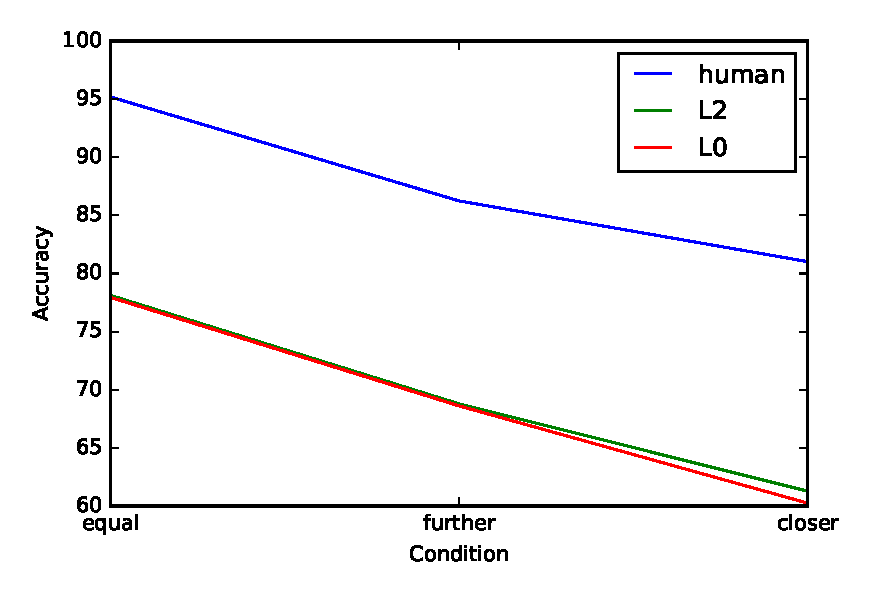
\includegraphics[scale = .5]{figures/allListenerAccuracy.eps}
\caption{Listener performance across conditions, for both human participants and model output}
\label{fig:listenerAccuracy}
\end{figure}

\subsection{Listener behavior}

Since color reference is a difficult task even for humans, we compared listener accuracy across conditions to calibrate our expectations about model performance. While participant accuracy was close to ceiling (95\%) on the `far' condition, they made many more errors on the `split' (86\%) and `close' (81\%) conditions (see Fig.~\ref{fig:listenerAccuracy}). 

\subsection{Speaker behavior}

For ease of comparison to computational results, we focus on five metrics capturing different aspects of the rich pragmatic behavior displayed by speakers in our task (see Table \ref{table:metrics}. 

\noindent{\bf Words and characters:} We counted the average number of words and characters per message, after removing stop words and punctuation. We found that participants used longer messages when distractors were closer to the target in color space.

\noindent{\bf Comparatives and superlatives:} We used the StanfordNLP POS tagger to count the number of comparatives (JJR or RBR) and superlatives (JJS or RBS) per message. We found that participants were more likely to use these constructions when one or more distractors were close to the target. Additionally, we found evidence of an asymmetry in the use of these constructions across the \emph{split} and \emph{close} conditions. Comparatives were used somewhat more often in the `split' condition, where only one distractor was close to the target, while superlatives were much more likely to be used in the `close' condition.

\noindent{\bf Negatives:} We counted occurrences of the string `not.' Participants were more likely to use negative constructions when one or more distractors were close to the target.

\begin{table}[t]
\centering
\begin{tabular}{lrr}
  \hline
  model & accuracy & perplexity \\
  \hline
  $\Listener_0$ & 69.0 & 3.04 \\
  $\Listener_2$ & \best{69.4} & \best{2.25} \\
  \hline
  human & 87.5 & -- \\
   \hline
\end{tabular}
\caption{Overall accuracy of the base listener, pragmatic listener, and human participants, plus model perplexity.}
\label{table:overallAccuracy}
\end{table}

\section{Model results}

\subsection{Listener accuracy}

We find that the pragmatic model is slightly more accurate at interpreting the
utterances of human speakers (\tabref{table:overallAccuracy}).

Breaking out the accuracy by condition (\figref{fig:listenerAccuracy}) reveals that
the primary gain from the pragmatic model is in the $close$ condition, when the
model has to pick up on the most subtle distinctions.

\begin{figure}
\centering
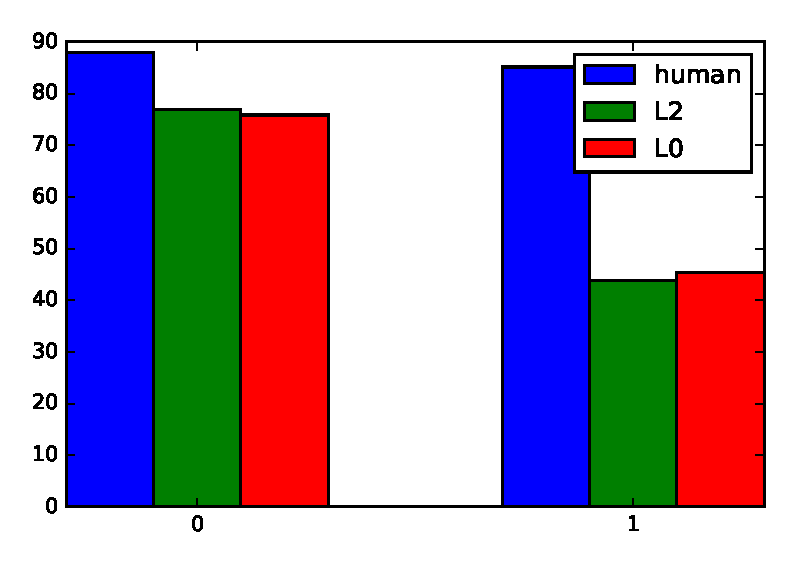
\includegraphics[width=0.8\columnwidth]{figures/byLength.eps}
\caption{Listener accuracy on utterances 6 words or less (``0'') and longer than
6 words (``1''), for both human participants and model outputs.}
\label{fig:byLength}
\end{figure}

We also see that the pragmatic model is more effective on shorter utterances
(\figref{fig:byLength}). This suggests that pragmatic considerations are more
important when the speaker is less informative.

\begin{table}[t]
\centering
\begin{tabular}{lrr}
  \hline
   & $\Listener_0$ & $\Listener_2$  \\
  \hline
  human        & 69.0 &       69.4  \\
  \hline
  $\Speaker_0$ & 73.3 &       73.1  \\
  $\Speaker_1$ & 80.0 & \best{80.2} \\
  \hline
\end{tabular}
\caption{Effectiveness of the speaker models communicating with the listener models,
measured by listener accuracy.}
\label{table:speakerVsListener}
\end{table}

\subsection{Speaker effectiveness}

\Tabref{table:speakerVsListener} shows the effectiveness of the two speaker models
(base speaker $\Speaker_0$ and pragmatic speaker $\Speaker_1$) at describing the
target color to the listener models.

The pragmatic speaker is better at communicating
with the listener models, which is unsurprising, because in the case of
$\Listener_0$, the speaker has access to the listener's thought process, and in
the case of $\Listener_2$, the listener has access to the speaker's thought process.

Additionally, however, the listeners are able to understand even $\Speaker_0$'s
utterances better than humans'. This is surprising, because $\Listener_0$ does not
contain an embedded model of either speaker, and $\Listener_2$ uses $\Speaker_0$
only indirectly, as a source of alternative utterances to consider.

\section{Related work}

\newcite{AndreasKlein16_NeuralPragmatics} also combine neural speaker and listener
models to model pragmatics. They implement and evaluate a pragmatic speaker
$\Speaker(\Listener_0)$, with sampling from a neural $\Speaker_0$ model to limit
the search space and regularize the model toward human-like utterances.

Our approach goes one step beyond theirs, in that we build a two-level derived
pragmatic model $\Listener(\Speaker(\Listener_0))$; i.e., we use a similar sampling
scheme to limit the search space in speaker modeling, and then explicitly normalize
over the colors in the context to derive a pragmatic listener.

Additionally, we use more powerful recurrent models for both the base speaker and the
base listener; \newcite{AndreasKlein16_NeuralPragmatics} use multi-layer perceptron
models over $n$-gram features. We also use a different strategy for blending the
pragmatic and base models: their model blends the base speaker and base listener
$\Speaker_0^{\beta} \cdot \Listener_0^{\beta}$ and
normalizes across utterances to implicitly define a different pragmatic model,
whereas we first compute the full normalized pragmatic
model $\Listener(\Speaker(\Listener_0))$ and blend it with a base listener by
$\Listener_0^{\beta} \cdot \Listener(\Speaker(\Listener_0))^{1 - \beta}$.

%\section{Credits}
%
%This document has been adapted from the instructions for ACL proceedings, including those for ACL-2008 by Johanna D. Moore, Simone Teufel, James Allan, and Sadaoki Furui, those for ACL-2005 by Hwee Tou Ng and Kemal Oflazer, those for ACL-2002 by Eugene Charniak and Dekang Lin, and earlier ACL and EACL formats. Those versions were written by several people, including John Chen, Henry S. Thompson and Donald Walker. Additional elements were taken from the formatting instructions of the {\em International Joint Conference on Artificial Intelligence}.
%
%\section{Introduction}
%
%The following instructions are directed to authors of papers submitted to TACL or accepted for publication. All authors are required to adhere to these specifications. Authors are required to provide a Portable Document Format (PDF)
%% das: removed reference to PostScript
%% and PostScript
%version of their papers. \textbf{The proceedings will be printed on
%US-Letter paper}. Authors from countries in which access to
%word-processing systems is limited should contact TACL editors at editors-in-chief@transacl.org as soon as possible.
%
%
%\section{General Instructions}
%
%Manuscripts must be in two-column format. Exceptions to the two-column format include the title,
%authors' names and complete addresses, which must be centered at the top of the first page,
%and any full-width figures or tables (see the guidelines in Subsection~\ref{ssec:first}). {\bf Type single-spaced}.
%Start all pages directly under the top margin. See the guide-lines later regarding formatting the first page. Do not number the pages.
%
%\subsection{Electronically-available resources}
%
%TACL provides this description in \LaTeX2e (tacl.tex) and PDF format (tacl.pdf), along with the LATEX2e style file used to format it (acl2012.sty) and an ACL bibliography style (acl2012.bst).  A Microsoft Word template file (tacl.dot) is also available. We require the use of these style files, which have been appropriately tailored for TACL. If you have an option, we recommend that you use the \LaTeX2e version. \textbf{If you will be using the Microsoft Word template, we suggest that you anonymize your source file so that the pdf produced does not retain your identity.} This can be done by removing any personal information from your source
%document properties.
%
%
%\subsection{Format of Electronic Manuscript}
%\label{sect:pdf}
%
%For the production of the electronic manuscript you must use Adobe's
%Portable Document Format (PDF). This format can be generated from
%postscript files: on Linux/Unix systems, you can use {\tt ps2pdf} for this
%purpose; under Microsoft Windows, you can use Adobe's Distiller, or
%if you have {\tt cygwin} installed, you can use {\tt dvipdf} or
%{\tt ps2pdf}.  Note
%that some word processing programs generate PDF which may not include
%all the necessary fonts (esp. tree diagrams, symbols). When you print
%or create the PDF file, there is usually an option in your printer
%setup to include none, all or just non-standard fonts.  Please make
%sure that you select the option of including ALL the fonts.  {\em Before sending it, test your PDF by printing it from a computer different from the one where it was created}. Moreover,
%some word processor may generate very large postscript/PDF files,
%where each page is rendered as an image. Such images may reproduce
%poorly.  In this case, try alternative ways to obtain the postscript
%and/or PDF.  One way on some systems is to install a driver for a
%postscript printer, send your document to the printer specifying
%``Output to a file'', then convert the file to PDF.
%
%Additionally, it is of utmost importance to specify the {\bf US-Letter format} (8.5in $\times$ 11in) when formatting the paper. When working with {\tt dvips}, for instance, one should specify {\tt -t letter}.
%
%Print-outs of the PDF file on US-Letter paper should be identical to the
%hardcopy version.  If you cannot meet the above requirements about the
%production of your electronic submission, please contact the
%publication chair above as soon as possible.
%
%
%\subsection{Layout}
%\label{ssec:layout}
%
%Format manuscripts two columns to a page, in the manner these
%instructions are formatted. The exact dimensions for a page on US-letter
%paper are:
%
%\begin{itemize}
%\item Left and right margins: 1in
%\item Top margin:1in
%\item Bottom margin: 1in
%\item Column width: 3.15in
%\item Column height: 9in
%\item Gap between columns: 0.2in
%\end{itemize}
%
%\noindent Papers should not be submitted on any other paper size. If you cannot meet the above requirements about the production of your electronic submission, please contact the publication chair above as soon as possible.
%
%\subsection{Fonts}
%
%For reasons of uniformity, Adobe's {\bf Times Roman} font should be
%used. In \LaTeX2e{} this is accomplished by putting
%
%\begin{quote}
%\begin{verbatim}
%\usepackage{times}
%\usepackage{latexsym}
%\end{verbatim}
%\end{quote}
%in the preamble. If Times Roman is unavailable, use {\bf Computer
%Modern Roman} (\LaTeX2e{}'s default).  Note that the latter is about
%10\% less dense than Adobe's Times Roman font.
%
%
%\begin{table}[h]
%\begin{center}
%\begin{tabular}{|l|rl|}
%\hline \bf Type of Text & \bf Font Size & \bf Style \\ \hline
%paper title & 15 pt & bold \\
%author names & 12 pt & bold \\
%author affiliation & 12 pt & \\
%the word ``Abstract'' & 12 pt & bold \\
%section titles & 12 pt & bold \\
%document text & 11 pt  &\\
%captions & 10 pt & \\
%abstract text & 10 pt & \\
%bibliography & 10 pt & \\
%footnotes & 9 pt & \\
%\hline
%\end{tabular}
%\end{center}
%\caption{\label{font-table} Font guide. }
%\end{table}
%
%\subsection{The First Page}
%\label{ssec:first}
%
%Center the title, author's name(s) and affiliation(s) across both
%columns. Do not use footnotes for affiliations.  Do not include the
%paper ID number assigned during the submission process.
%Use the two-column format only when you begin the abstract.
%
%{\bf Title}: Place the title centered at the top of the first page, in
%a 15 point bold font.  (For a complete guide to font sizes and styles, see Table~\ref{font-table}.)
%Long title should be typed on two lines without
%a blank line intervening. Approximately, put the title at 1in from the
%top of the page, followed by a blank line, then the author's names(s),
%and the affiliation on the following line.  Do not use only initials
%for given names (middle initials are allowed). Do not format surnames
%in all capitals (e.g., ``Zhou,'' not ``ZHOU'').  The affiliation should
%contain the author's complete address, and if possible an electronic
%mail address. Leave about 0.75in between the affiliation and the body
%of the first page. The title, author names and addresses should be completely identical to those entered to the electronic paper submission website in order to maintain the consistency of author information among all publications of the conference.
%
%{\bf Abstract}: Type the abstract at the beginning of the first
%column.  The width of the abstract text should be smaller than the
%width of the columns for the text in the body of the paper by about
%0.25in on each side.  Center the word {\bf Abstract} in a 12 point
%bold font above the body of the abstract. The abstract should be a
%concise summary of the general thesis and conclusions of the paper.
%It should be no longer than 200 words. The abstract text should be in 10 point font.
%
%{\bf Text}: Begin typing the main body of the text immediately after
%the abstract, observing the two-column format as shown in
%the present document. Do not include page numbers.
%
%{\bf Indent} when starting a new paragraph. For reasons of uniformity,
%use Adobe's {\bf Times Roman} fonts, with 11 points for text and
%subsection headings, 12 points for section headings and 15 points for
%the title.  If Times Roman is unavailable, use {\bf Computer Modern
%Roman} (\LaTeX2e's default; see section \ref{sect:pdf} above).
%Note that the latter is about 10\% less dense than Adobe's Times Roman
%font.
%
%\subsection{Sections}
%
%{\bf Headings}: Type and label section and subsection headings in the
%style shown on the present document.  Use numbered sections (Arabic
%numerals) in order to facilitate cross references. Number subsections
%with the section number and the subsection number separated by a dot,
%in Arabic numerals. Do not number subsubsections.
%
%{\bf Citations}: Citations within the text appear
%in parentheses as~\cite{Gusfield:97} or, if the author's name appears in
%the text itself, as Gusfield~\shortcite{Gusfield:97}. Append lowercase letters to the year in cases of ambiguities. Treat double authors as in~\cite{Aho:72}, but write as in~\cite{Chandra:81} when more than two authors are involved. Collapse multiple citations as in~\cite{Gusfield:97,Aho:72}. Also refrain from using full citations as sentence constituents. We suggest that instead of
%\begin{quote}
%``\cite{Gusfield:97} showed that ...''
%\end{quote}
%you use
%\begin{quote}
%``Gusfield \shortcite{Gusfield:97}   showed that ...''
%\end{quote}
%
%If you are using the provided \LaTeX{} and Bib\TeX{} style files, you
%can use the command \verb|\newcite| to get ``author (year)'' citations.
%
%As reviewing will be double-blind (except that action editors know author identity and authors know action-editor identity), the submitted version of the papers should not include the
%authors' names and affiliations. Furthermore, self-references that
%reveal the author's identity, e.g.,
%\begin{quote}
%``We previously showed \cite{Gusfield:97} ...''
%\end{quote}
%should be avoided. Instead, use citations such as
%\begin{quote}
%``Gusfield \shortcite{Gusfield:97}
%previously showed ... ''
%\end{quote}
%
%To be clear: You should reference your prior work if it is relevant; but use the third person instead of the 1st person and in place of references like “(Anonymous) showed…”, since such anonymized references do not allow readers to examine relevant related work.
%
%Authors’ names should also be removed from the ``Document Properties'' display that can be viewed using Adobe Acrobat’s ``File $\rightarrow$ Properties'' menu.
%
%Please do not include acknowledgements when submitting your papers. Papers that do not conform
%to these requirements may be rejected without review.
%
%\textbf{References}: Gather the full set of references together under
%the heading {\bf References}; place the section before any Appendices,
%unless they contain references. Arrange the references alphabetically
%by first author, rather than by order of occurrence in the text.
%Provide as complete a citation as possible, using a consistent format,
%such as the one for {\em Computational Linguistics\/} or the one in the
%{\em Publication Manual of the American
%Psychological Association\/}~\cite{APA:83}.  Use of full names for
%authors rather than initials is preferred.  A list of abbreviations
%for common computer science journals can be found in the ACM
%{\em Computing Reviews\/}~\cite{ACM:83}.
%
%The \LaTeX{} and Bib\TeX{} style files provided roughly fit the
%American Psychological Association format, allowing regular citations,
%short citations and multiple citations as described above.
%
%{\bf Appendices}: Appendices, if any, directly follow the text and the
%references (but see above).  Letter them in sequence and provide an
%informative title: {\bf Appendix A. Title of Appendix}.
%
%\textbf{Acknowledgment} sections should go as a last section immediately
%before the references. Do not number the acknowledgement section.
%
%\subsection{Footnotes}
%
%{\bf Footnotes}: Put footnotes at the bottom of the page. They may
%be numbered or referred to by asterisks or other
%symbols.\footnote{This is how a footnote should appear.} Footnotes
%should be separated from the text by a line.\footnote{Note the
%line separating the footnotes from the text.}  Footnotes should be in 9 point font.
%
%\subsection{Graphics}
%
%{\bf Illustrations}: Place figures, tables, and photographs in the
%paper near where they are first discussed, rather than at the end, if
%possible.  Wide illustrations may run across both columns and should be placed at
%the top of a page. Color illustrations are discouraged, unless you have verified that
%they will be understandable when printed in black ink.
%
%{\bf Captions}: Provide a caption for every illustration; number each one
%sequentially in the form:  ``Figure 1. Caption of the Figure.'' ``Table 1.
%Caption of the Table.''  Type the captions of the figures and
%tables below the body, using 10 point text.
%
%\section{Translation of non-English Terms}
%
%It is also advised to supplement non-English characters and terms
%with appropriate transliterations and/or translations
%since not all readers understand all such characters and terms.
%
%Inline transliteration or translation can be represented in
%the order of: original-form transliteration ``translation''.
%
%\section{Length of Submission}
%\label{sec:length}
%
%Submissions may consist of seven to ten (7-10) letter format (not A4) pages of content and unlimited additional pages (only) allowed for references. Papers that are revisions of submissions with prior (b) or (c) decisions may be allowed one to two additional pages of content to accommodate required revisions.
%
%Appendices (if any) are counted as content pages. Papers that do not conform to the specified length and
%formatting requirements are subject to re-submission.
%

\section*{Acknowledgments}

Do not number the acknowledgment section. Do not include this section when submitting your paper for review.

\bibliography{colors}
\bibliographystyle{acl2012.bst}

\end{document}



